\chapter{Characterizing the Two-Qubit Processor} \label{chapter:processor_characterization}

After having detailed the design of the processor and the measurement techniques employed in this work, we will now show how we can ``test drive'' it to show the basic functionality that we need to run meaningful quantum algorithms. In particular we show how we can implement a robust two-qubit quantum gate that we will use in the following chapter to run a real-world quantum algorithm on our processor.

\smallskip

We begin the chapter by discussing the measurement of the basic qubit and readout parameters. We will then give a detailed overview of the relevant decoherence times and readout fidelities of our processor at different working points and discuss our strategy for optimizing these parameters during the operation of the processor. Afteward we will explain the realization of single-qubit gates together with possible error sources that we need to take into account. We also discuss in detail the generation and characterization of entanglement. Finally, we discuss the implementation of a universal two-qubit gate and its characterization through quantum process tomography.

\section{Qubit \& Readout Characterization}

\begin{figure}[ht!]
	\centering
		\includegraphics[width=1.\textwidth]{"./data/ct5/qubit frequencies/qubit_spectroscopy"}
	\label{fig:ProcessorSpectroscopy}
	\caption[Spectroscopy of the Two-Qubit Processor]{Spectroscopy of our two-qubit processor. Shown are the $\ket{0}\to\ket{1}$ ($\omega_{01}$) and $(\ket{0}\to\ket{2})/2$ ($\omega_{02}/2$) transition frequencies of the two qubits, together with a fitted analytical model of the qubit parameters. We also show the frequencies of the two readout resonators. The frequencies $f_M^{I}$ and $F_M^{II}$ indicate the working points of the qubits for single-qubit manipulation \figcomment{add more information to the figure and correct the notation of the manipulation working point}}
\end{figure}

The first step in the characterization of the processor consists in obtaining all the relevant qubit and readout parameters. For this, we perform a set of measurements from which we obtain the qubit frequencies, anharmonicities, junction asymmetries, the inter-qubit coupling, the coupling to the microwave drive lines, the coupling of each qubit to its readout and the relaxation and dephasing times of the qubits. Most of these parameters, such as the drive and readout couplings as well as the relaxation and dephasing times are measured for a range of qubit frequencies, which will allow us later to pick an ideal working point for our two-qubit experiments. A detailed account of the spectroscopic techniques employed here can be found in chapter \ref{chapter:measurement}. The qubit parameters that we obtain from our measurements are as follows:

\subsubsection{Qubit Parameters}

To obtain the Josephson and charging energies as well as the junction asymmetries of the qubits we perform spectroscopic measurements of the single-photo n$\ket{0}\to \ket{1}$ and the two-photon $\ket{0}\to\ket{2}$ qubit transitions at different values of the magnetic flux $\Phi$. Fitting the resulting values $\omega_{01}(\Phi)$ and $\omega_{20}(\Phi)$ to a theoretical model we obtain all relevant qubit parameters. For our processor, these are $E_J^I / h = 36.2\; \mathrm{GHz}$, $E_c^I / h = 0.98 \; \mathrm{GHz}$ and $E_J^{II} / h = 43.1\; \mathrm{GHz}$, $E_C^{II} / h = 0.87 \; \mathrm{GHz}$ for the Josephson and charging energies of the two qubits and $d^I = 0.2$, $d^{II} =  0.35$ for the qubit junction asymmetries.

\subsubsection{Readout Parameters}

To obtain the resonance frequencies and quality factors of the readout resonators we perform a simple reflectometric measurement of the $S_{11}$ transmission coefficient of the resonators. The resulting frequencies are $\nu_R^I = 6.84 \; \mathrm{GHz}$ and $\nu_R^{II} = 6.70 \; \mathrm{GHz}$ with quality factors $Q^I \simeq Q^{II} = 730$. We measure the Kerr nonlinearity $K$ of the resonators by following the procedure given in \citep[p. 166]{palacios-laloy_superconducting_2010} and obtain $K^I / \nu_R^I \simeq K^{II} / \nu_R^{II} = -2.3\pm 0.5 \times 10^{-5}$ 

\subsubsection{Qubit/Readout Couping}

The coupling of the qubits to the readout resonators can be determined by spectroscopically measuring the avoided level crossing between the two systems. For this, we perform a series of spectroscopic measurements of the resonator for a range of qubit frequencies ranging from below the resonator frequency to above it. The results of these measurements are shown in fig. \ref{fig:qubit_resonator_anticrossing} and cleary show an avoided level crossing between the two systems. From the width of this crossing we can obtain the qubit-resoantor coupling coefficients, which are $g_0^I \simeq g_0^{II} = 50 \; \mathrm{MHz}$.

\begin{figure}[htb!]
	\centering
	\includegraphics[width=1\textwidth]{"./data/ct5/cavity anticrossing/qubits_anticrossing_bw"}
	\caption[Spectroscopic measurement of the avoided level crossing between the two qubits and their corresponding readout resonator]{Spectroscopic measurement of the avoided level crossing between the two qubits and their corresponding readout resonator, corresponding to an effective qubit-resonator coupling strength $2g\approx 50\;\mathrm{MHz}$.}
	\label{fig:qubit_resonator_anticrossing}
\end{figure}


\subsubsection{Qubit Parameter Survey}

\begin{figure}[ht!]
   \centering
	 \includegraphics[width=1\textwidth]{"./data/ct5/qubits - parameter surveys/qubit parameters"}
	 \caption[A qubit parameter survey showing $T_1$, readout contrast and Rabi frequency of the two qubits over a large range of qubit frequencies]{A qubit parameter survey showing the relaxation time $T_1$, the readout contrast and the Rabi frequency at a fixed drive amplitude for the two qubits over a large range of qubit frequencies.}
	 \label{fig:qubit_parameters}
\end{figure}

In order to determine the optimal working point for our processor we need to characterize the properties of the qubits at many different frequencies. For this, we perform an automated survey where we measure the transition frequencies $\omega_{01}$ and $\omega_{20}$, the readout contrast $c$ and the relaxation and dephasing times $T_1$ and $T_2$ of each qubit at different values of the magnetic flux $\Phi$. The results of such a parameter survey are summarized in fig \ref{fig:qubit_parameters}, where we show the relaxation time $T_1$,  the readout contrast $c_{10}$ and the Rabi frequency $f_{Rabi}$ at fixed drive amplitude for the two qubits within a frequency range between 5.2 and 6.5 GHz. As can be seen, the relaxation time of the qubits tends to increase the farther detuned each qubit is from its readout resonator. Not surprisingly, the drive frequency of the qubit also decreases when the qubit-resonator detuning increases, as expected from the so-called {\it Purcell effect}, which filters incoming microwave signals that are far-detuned from the resonator frequency. The inverse is true for the readout contrast, which increases nearly linear when reducing the qubit-resonator detuning. This can be explained by the increase of the dispersive resonator frequency shift $\chi$induced by the qubit, which decreases with the detuning $\Delta$ roughly as $1/\Delta$(???).

\smallskip

It is interesting to note the non-monotonous characteristic of the qubit relaxation time $T_1$ shown in fig. \ref{fig:qubit_parameters}, which cannot be explained by Purcell-filtering through the readout resonator and hints thus at a different qubit relaxation process present in the system. A possible explanation would be the coupling of the qubit to spurious low-Q resonances in the environment. For example, the coupling of the qubit to volumetric resonance modes of the sample holder or to non-CPW resonance modes of the readout resonator could be possible explanations for the data. Also, the overall dependency of the relaxation time $T_1$ on the qubit-resonator detuning --ignoring the ``fine-structure'' present in the system-- is not quadratic as would be expected from the Purcell theory but rather linear. Also, by comparing the qubit relaxation time to the Rabi drive frequency reveals that the increase in $T_1$ is clearly not proportional to the Purcell factor, that determines both the qubit relaxation rate through the readout resonator and the Rabi drive frequency. However, the observed $T_1$ dependency can be partially explained by taking into account the qubit relaxation through the fast fluxline, which might be too strongly coupled to the qubit, hence inducing additional qubit relaxation beyond the Purcell and intrinsic qubit relaxation rates.

\section{Single-Qubit Operations}

\begin{figure}[ht!]
	\centering
		\includegraphics[width=1.\textwidth]{"./data/ct5/2010_12_01 - iq tomography/iq_tomographies"}
	\caption[Demonstration of single-qubit IQ control]{Demonstration of single-qubit IQ control. The figures show the state probability of a single qubit when preparing it in one of the states $\ket{1}$, $1/\sqrt{2}(\ket{0}+\ket{1})$ or $1/\sqrt{2}(\ket{0}+i\ket{1})$ and subjecting the qubit to a microwave drive pulse of the form $a(t) = V_I\cdot\cos{\omega_{rf}t}+V_Q\cdot\sin{\omega_{rf}t}$ of varying amplitudes $V_I$ and $V_Q$ and constant duration.}
	\label{fig:single_qubit_iq_control}
\end{figure}

To perform arbitrary single-qubit operations -- as needed e.g. for implementing a quantum algorithm or performing quantum state tomography -- we need to implement a universal set of $X$, $Y$ and $Z$ qubit gates on our processor. Qubit rotations in the $XY$-plane are implemented through microwave drive pulses, where the phase of the drive pulse in reference to an arbitrary reference determines the rotation axis and the amplitude of the drive pulse the Rabi frequency of the gate. To characterize the drive pulses, we perform an experiment where we initialize a single-qubit in the states $\ket{1}$, $1/\sqrt{2}(\ket{0}+\ket{1})$ and $\sqrt{2}(\ket{0}+i\ket{1})$ and subject it afterward to a single microwave pulse of the form $a(t) = V_I\cdot\cos{\omega_{rf}t}+V_Q\cdot\sin{\omega_{rf}t}$, which we tune by changing the input voltages $V_I$ and $V_Q$ to the $IQ$-mixer that generates the pulse from a continuous input microwave-tone at frequency $\omega_{rf}$. We measure the qubit state at different values of $V_I$, $V_Q$, obtaining the graph shown in fig. \ref{fig:single_qubit_iq_control}. The qubit which was prepared in state $\ket{1}$ shows a perfectly cylinder-symmetric switching probability pattern when subjecting it to an IQ-pulse of a given phase, which is what one would expect for a qubit being prepared in either the $\ket{0}$ or $\ket{1}$ state. On the contrary, the switching probability distributions of the measured qubits prepared in the states $1/\sqrt{2}(\ket{0}+\ket{1})$ and $1/\sqrt{2}(\ket{0}+i\ket{1})$ are mirror-symmetric, where the switching probability does not vary at all along the drive axis that corresponds to the axis along which the qubit has been prepared. These measurements demonstrate therefore our ability to prepare and drive the qubit along arbitrary axes of the Bloch sphere. In the following sections we will analyze more in detail the drive errors inherent to our system and quantitatively analyze different error sources. 

\subsection{Estimation of drive errors}

\begin{figure}[htp!]
	\centering
	\includegraphics[width=\textwidth]{"./material/mathematica/three_level_driving_errors"}
	\caption[Single-qubit $\pi$-pulse gate time, gate fidelity and AC stark detuning as a function of drive strength]{The single-qubit $\pi$-pulse gate time, gate fidelity and AC stark detuning, plotted as a function of the drive strength $\epsilon$ applied to the three-level Transmon. As the drive strength increases, the gate time decreases as $1/\epsilon$ whereas the gate fidelity decreases approximately quadratically.}
	\label{fig:three_level_driving_errors}
\end{figure}

Since the Transmon is a weakly anharmonic multi-level system and thus no real qubit, driving the $\ket{0}\to\ket{1}$ transition with high power can induce transitions to higher Transmon levels. It is important to estimate and reduce these errors when performing fast qubit gates e.g. for state preparation or tomography. To model the driving of a Transmon, we use the simple drive model in the rotating-frame approximation and as used e.g. in \cite{motzoi_simple_2009}:
%
\begin{equation}
\hat{H} = \left(
						 \begin{array}{ccc}
						0 & \epsilon^*(t) & 0 \\
						\epsilon(t) & \delta & \sqrt{2}\epsilon^*(t) \\
						0 & \sqrt{2}\epsilon(t) & 2\delta + \alpha
						\end{array}
					\right) \label{eq:qubit_three_level_driving_hamiltonian}
\end{equation}
%
Here, $\epsilon(t) = \epsilon_x(t)+i\epsilon_y(t)$ is the complex drive IQ amplitude in the rotating qubit frame, $\delta$ is the detuning of the microwave drive from the Transmon $\omega_{01}$ transition frequency and $\alpha$ is the Transmon anharmonicity. To estimate the leakage to higher Transmon levels, we calculate the eigenvalues and eigenvectors of the Hamiltonian given in eq. (\ref{eq:qubit_three_level_driving_hamiltonian}). We then decompose an initial state $\ket{0}$ in the basis of eigenstates and let it evolve under a given constant drive amplitude $\epsilon_0$. By maximizing the occupation probability of the state $\ket{1}$ as a function of the evolution time and drive detuning $\delta$ we obtain the gate time, state fidelity and AC-Stark shift for the applied drive strength. These quantities are shown in fig. \ref{fig:three_level_driving_errors}, which shows the numerically obtained gate time, gate fidelity and AC-stark shift of the qubit frequency as a function of the applied drive frequency. As can be seen, the gate error increases almost quadratically with the drive frequency. Typically, in our experiments we use drive frequencies between 100 - 200 MHz, inducing thus single-qubit drive errors between 1-3 \%. In general, it is possible to correct these errors using optimized drive pulses \cite{lucero_reduced_2010,chow_optimized_2010}, thereby eliminating leakage to the third qubit level. In this work, we did not use such techniques but we will  include possible errors arising due to this leakage to higher Transmon levels in our error models when discussing our experimental data.

\section{Two Qubit Operations}

\begin{figure}[ht!]
	\centering
		\includegraphics[width=0.7\textwidth]{"./data/ct5/2011_04_11 - anticrossing/qubit_anticrossing_modified"}
	\caption[Spectroscopic measurement of the avoided level crossing between the two qubits of our processor]{a) Spectroscopy measurement of the avoided level crossing between the two qubits of our processor. b) Single spectroscopy of qubit I when in resonance with qubit II. From this spectroscopic measurement, a qubit-qubit strength of $2g=8.9\;\mathrm{MHz}$ can be deduced. }
	\label{fig:qubit_anticrossing}
\end{figure}

We use the capacitive coupling between the qubits to implement two-qubit gates and create entangled states between the two qubits. To characterize the qubit-qubit interaction, we first perform a spectroscopic measurement of the system. For this, we measure a spectroscopy of one of the qubits for a range of qubit frequencies such that the frequency of qubit I, $\omega_{01}^I$ gets tuned through the frequency of qubit II, $\omega_{01}^{II}$. When these two frequencies are sufficiently close we observe an avoided level crossing between the qubits. At resonance, the gap between the two spectroscopic lines that appear corresponds to the qubit-qubit coupling strength $2g$. Fig \ref{fig:qubit_anticrossing} shows the results of such a measurement, qubit II was positioned at a $5.125\;\mathrm{GHz}$ and the frequency of qubit II was tuned from $5.1-5.15\;\mathrm{GHz}$. At resonance we measure a coupling strength of $2g = 8.3\;\mathrm{MHz}$.

\smallskip

If the two qubit frequencies $\omega_{01}^I$, $\omega_{01}^{II}$ are far detuned such that $|\omega_{01}^I-\omega_{01}^{II}|\gg 2g$, the eigenstates of the coupled two-qubit Hamiltonian correspond to a very good accuracy to the independent qubit states $\ket{01}$ and $\ket{10}$. Therefore, far from the resonance we observe only one spectroscopic line corresponding to the transition $\ket{00}\to\ket{10}$ (since we drive only the first qubit). However, close to resonance the eigenstates approach the Bell states $\ket{\Psi_\pm} = 1/\sqrt{2}(\ket{10}\pm\ket{01})$, which can both be excited by driving qubit I. Hence we observe two spectroscopic lines corresponding to the two transition $\ket{00}\to 1/\sqrt{2}(\ket{01}+\ket{10})$ and $\ket{00}\to 1/\sqrt{2}(\ket{01}-\ket{10})$. 

\subsection{Creation of Entanglement} \label{section:creation_of_entanglement}

\begin{SCfigure}[1][ht!]
	\centering
	\includegraphics[width=0.6\textwidth]{"./material/figures/measurement/qubit_swap"}
	\caption[Pulse sequence used to create an entangled two-qubit state]{Pulse sequence used to create an entangled two-qubit state using a non-adiabatic transfer from an off-resonant to a resonant two-qubit state.}
	\label{fig:qubit_swap_pulse_sequence}
\end{SCfigure}

After having characterized the qubit-qubit interaction using a spectroscopic measurement we perform a coherent swapping operation between the qubits. We implement this operation by non-adiabatically changing the resonance frequency of the qubits from an off-resonance to an on-resonance condition. When doing this after preparing the qubits in one of the states $\ket{01}$ or $\ket{10}$ we induce a coherent energy swap between the qubits. We then terminate the interaction after a well-defined time and measure the state of the two-qubit register directly afterward. When the qubits are in resonance, the time evolution operator of their quantum state is given as
%
\begin{equation}
U(t)=\left(\begin{array}{cccc}
1 & 0 & 0 & 0\\
0 & \cos{2\pi tg} & i\sin{2\pi tg} & 0\\
0 & i\sin{2\pi tg} & \cos{2\pi tg} & 0\\
0 & 0 & 0 & 1\end{array}\right)_{\left\{ \left|00\right\rangle ,\left|01\right\rangle ,\left|10\right\rangle ,\left|11\right\rangle \right\} } \label{eq:swap_evolution_operator_main}
\end{equation}
%
As can be seen, the two basis states $\ket{01}$ and $\ket{10}$ oscillate back and forth between each other with frequency $g$. The states $\ket{00}$ and $\ket{11}$ are not affected by the interaction.

\smallskip

\begin{figure}[ht!]
	\centering
	\includegraphics[width=0.7\textwidth]{"./material/papers/iswap/figures/swap_raw_and_corrected"}
	\caption[]{State occupation probabilities for the two-qubit register during a coherent energy swap. a) Shows the raw state probabilities corresponding to the states $\ket{00}$, $\ket{01}$, $\ket{10}$ and $\ket{11}$, b) shows the same data corrected for the limited visibility of each qubit readout and c) shows the fully corrected readout data where we account for both visibility and inter-qubit readout crosstalk errors.}
	\label{fig:swap_raw_and_corrected}
\end{figure}

Fig. \ref{fig:qubit_swap_pulse_sequence} summarizes the frequency, drive and measurement pulse sequence that we use for this experiment. When varying the time during which the qubits are in resonance we can observe the coherent swapping of energy between them. Figure \ref{fig:swap_raw_and_corrected} presents the results of such a measurement. Shown are the measured qubit state probabilities $p(\ket{00})$, $p(\ket{01})$, $p(\ket{10})$ and $p(\ket{11})$ as a function of the swap duration $\Delta t$. Subfigure a) shows the raw, uncorrected readout data, subfigure b) shows the probabilities corrected for limited readout visibility and subfigure c) shown the probabilities corrected for both limited readout visibility and inter-readout crosstalk. The osciallatory behavior between the states $\ket{01}$ and $\ket{10}$ is well-visible in the data. Also, the frequency of the energy swap $2g=8.3\;\mathrm{MHz}$ agrees well with the value obtained from the spectroscopic measurement. Fig. \ref{fig:swap_raw_and_corrected}c shows, in addition to the measured state occupation probabilities, a master equation simulation of the experiment. This simulation takes into account relaxation and dephasing of the qubits. The relaxation rates used in the simulation correspond to the experimentally measured relaxation rates at the operating frequencies of the qubits, whereas the dephasing rates were free fitting parameters. We do not use the measured single-qubit dephasing times in our simulation since they do not correspond to the effective dephasing rate of the two-qubit system at resonance, which cannot be described within the master equation formalism. The reason for this is that the transition frequency of the two eigenstates $\ket{\phi_\pm}=1/\sqrt{2}(\ket{01}\pm\ket{10})$ at resonance $\omega_{01}^{\pm}=\omega_{01}^{I,II}\pm\sqrt{4g^2+\Delta^2}/2\approx \omega_{01}^{I,II}\pm g +\Delta^2/8g$ is insensitive to variations of $\Delta$ to first order. Hence, the effective dephasing rate of the two-qubit system will be much higher than the single-qubit dephasing rates. To reproduce the experimentally observed dephasing we therefore use effective dephasing rates $\Gamma_\phi^{I,II}=2\;\mathrm{\mu s}$ in our simulation. As can be seen, using these rates and the measured relaxation rates and coupling parameter the simulation agrees very well with the experimental data.

\subsection{Quantum State Tomography}

The experiments that we describe in the following sections often require us to determine the density matrix of an experimental two-qubit state. The method that we use for this purpose is called {\it quantum state tomography} (QST) (see e.g. \cite{nielsen_quantum_2000} for an overview of this method). In this section, we therefore explain in detail the procedure that we use to perform QST. Furthermore, we also discuss several sources of errors occurring in standard QST and how we can estimate their effect on our results.

\smallskip

The density matrix of an n-qubit system can be written as
%
\begin{eqnarray}
\rho & = & \sum\limits_{v_1,v_2\hdots v_n} \frac{c_{v_1,v_2\hdots v_n} \sigma_{v_1}\otimes \sigma_{v_2}\hdots \sigma_{v_n}}{2^n} \label{eq:state_tomography_state_representation} \\
c_{v_1,v_2\hdots v_n} & = & \mathrm{Tr}\left\{\sigma_{v_1}\otimes \sigma_{v_2}\hdots \otimes\sigma_{v_n} \; \rho \right\} \label{eq:state_tomography_coefficients}
\end{eqnarray}
%
where $v_i \in \left\{ X,Y,Z,I\right\}$ and $n$ gives the number of qubits in the system and where the $c_{v_1,v_2\hdots v_n}$ are real-valued coefficients that describe the given density matrix. To reconstruct the density matrix of an experimental quantum system in a well-prepared state it is thus sufficient to measure the expectation values of these $n^2-1$ coefficients on an ensemble of identically prepared states. For our two qubit system, this means measuring all possible combinations of the operators $\{I,\sigma_x^I,\sigma_y^I,\sigma_z^I\}\otimes\{I,\sigma_x^{II},\sigma_y^{II},\sigma_z^{II}\}$. However, in our experiments, rather than measuring $\sigma_x$ and $\sigma_z$ operators directly, we rotate the quantum state of each qubit around such that the state vector along the desired measurement axis coincides with the z-axis of the Bloch sphere and measure $\sigma_z$ afterward.

When using this direct measurement method, statistical and systematic measurement errors can yield a set of coefficients $v_i$ that corresponds to a {\it non-physical} density matrix, which violates either the positivity $\bra{\psi}\rho\ket{\psi} > 0$ (for all valid states $\ket{\psi}$) or the unity-trace condition $\mathrm{Tr}(\rho)=1$. To alleviate this problem, several techniques can be employed. In the following section we discuss an estimation technique which is able to overcome the problem of non-physical density matrices, the so-called {\it maximum likelihood estimation}.
When using this direct measurement method, statistical and systematic measurement errors can yield a set of coefficients $v_i$ that corresponds to a {\it non-physical} density matrix, which violates either the positivity $\bra{\psi}\rho\ket{\psi} > 0$ (for all valid states $\ket{\psi}$) or the unity-trace condition $\mathrm{Tr}(\rho)=1$. To alleviate this problem, several techniques can be employed. In the following section we discuss an estimation technique which is able to overcome the problem of non-physical density matrices, the so-called {\it maximum likelihood estimation}.

\subsubsection{Maximum Likelihood Estimation of Quantum States}

Maximum likelihood estimation is a method that numerically or analytically maximizes a likelihood function that is based on a number of measured outcomes and and a set of parameters that need to be estimated. The set of parameters that corresponds to the maximum of the probability function can then be interpreted as the one with the highest probability of generating the observed outcomes. When estimating the parameters of a density matrix with this method, the probability function to be maximized is the joint probability of obtaining the measured values $\{c_{X,X,\hdots,X},c_{Y,X,\hdots,X},\hdots,c_{I,I,\hdots,I}\}$ for a given density matrix $\hat{\rho}$. By numerically or analytically maximizing this joint probability over the set of possible density matrices we obtain the density matrix which is most likely to have produced the set of measurement outcomes that we have observed.

The joint measurement operators $\Sigma_j = \sigma_{v_1}\otimes \sigma_{v_2}\hdots \otimes\sigma_{v_n}$ have the eigenvalues $\pm 1$ and can thus be written as 
\begin{equation}
\sigma_{v_1}\otimes \sigma_{v_2}\hdots \otimes\sigma_{v_n} = \ket{+_j}\bra{+_j}-\ket{-_j}\bra{-_j} \label{eq:ml_operators}
\end{equation}
where $\ket{-_j}$ and $\ket{-_j}$ are the eigenstates corresponding to the eigenvalues $\pm 1$ of $\Sigma_j$. When performing $l$ measurements of the operator $\Sigma_j$, the expectation value $\langle \Sigma_j \rangle$ can be calculated as
%
\begin{equation}
\widehat{\langle \Sigma_j \rangle}_\rho = \frac{1}{l}\sum\limits_{i = 1}^l M_i(\Sigma_j,\rho) \label{eq:tomography_measurement_estimator}
\end{equation}
where $M_i(\Sigma,\rho)$ denotes the outcome of the $i$-th measurement of the operator $\Sigma$ on the state described by the density matrix $\rho$. Since each outcome $M_i(\Sigma_j,\rho)$ is Bernoulli distributed, the sum $\langle\hat{\Sigma_j}\rangle_\rho$ of them is binomially distributed with an expectation value \mbox{$E(\widehat{\langle \Sigma_j \rangle}_\rho) = \langle \Sigma_j \rangle_\rho$} and the variance $\sigma^2(\widehat{\langle \Sigma_j \rangle}_\rho) = 1/l \cdot (1-\langle \Sigma_j \rangle_\rho^2)$. For large sample sizes $l$, the binomial distribution can be well approximated by a normal distribution with the same expectation value and variance. The joint probability of obtaining a set of measurement values $\{s_1,\hdots,s_{n^2-1}\}$ for the set of operators $\{\widehat{\langle\Sigma_1 \rangle}_\rho,\hdots,\widehat{\langle\Sigma_{n^2-1} \rangle}_\rho\}$ is thus given as
%
\begin{equation}
P\left(\widehat{\langle \Sigma_1 \rangle }_\rho = s_1;\hdots;\widehat{\langle \Sigma_{n^2-1} \rangle}_\rho =  s_{n^2-1}\right) = \prod\limits_{i = 1}^{n^2-1} \exp{\left(-\frac{l}{2}\frac{(s_i-\langle \Sigma_i \rangle_\rho)^2}{1-\langle \Sigma_i \rangle_\rho^2}\right)}
\end{equation}
%
By maximizing this probability (or the logarithm of it) we obtain an estimate of the parameters of the density matrix $\rho$ of the quantum state. 

\subsubsection{Including Experimental Tomography Errors}

This technique also allows us to include further optimization parameters when calculating the joint probability. This is useful for modeling e.g. systematic errors of the measurement or preparation process, which can be described by modifying the operators contained in the probability sum. A common source of errors in our tomography measurements are shifts in the amplitude and phase of the microwave pulses used to drive the qubit. We are obliged to rotate the qubit state when performing state tomography since our measurement apparatus permits us only to measure the $\sigma_z$ operator of each qubit. We can therefore replace the operators $\sigma_x$ and $\sigma_y$ in eq. (\ref{eq:ml_operators}) with an effective measurement of $\sigma_z$ preceded by a rotation $R_{\nu_i}$ given as
\begin{eqnarray}
R_{X} & = & \exp{\left( -i \sigma_y \pi / 4\right)} \\
R_{Y} & = & \exp{\left( +i \sigma_x \pi / 4\right)} 
\end{eqnarray}
Within this model, phase and amplitude errors can be modeled by including additional phase factors in the exponential of these expression, such that we obtain new operators
\begin{eqnarray}
R_{X}' & = & \exp{\left( -i \left[+\sigma_y\cos{\alpha}+\sigma_x\sin{\alpha} \right] \left[\pi / 4+\gamma\right]\right)} \\
R_{Y}' & = & \exp{\left( +i \left[-\sigma_y\sin{\beta}+\sigma_x\cos{\beta}\right] \left[\pi / 4+\delta\right]\right)} 
\end{eqnarray}
Here, $\alpha$ and $\beta$ represent phase errors whereas $\gamma$ and $\delta$ represent amplitude errors in the drive pulses. An detailed discussion of how we fit these parameters in our experiment will be given in section \ref{section:tomographic_errors}.

\subsection{Creation of Bell states}

\begin{SCfigure}[1.0][ht!]
	\centering
	\includegraphics[width=9cm]{"./material/figures/measurement/bell_state_creation"}
	\caption[]{Pulse sequence used to experimentally generate entangled Bell states. The sequence consists in exciting one of the qubits to the state $\ket{1}$, creating an entangled state using the swapping interaction and correcting the acquired phase of the state. For the $\ket{\Phi_\pm}$ states, we use an additional $Y(\pi)$ pulse at the end of the sequence.}
	\label{fig:bell_generation_pulse_sequence}
\end{SCfigure}

We can use the ML method presented above to perform state tomography of entangled Bell states that we create by using the swapping interaction between the qubits. In general, the four Bell states are
%
\begin{eqnarray}
\ket{\Psi_+} = \frac{1}{\sqrt{2}}\left(\ket{01}+\ket{10}\right) \\
\ket{\Psi_-} = \frac{1}{\sqrt{2}}\left(\ket{01}-\ket{10}\right) \\
\ket{\Phi_+} = \frac{1}{\sqrt{2}}\left(\ket{00}+\ket{11}\right) \\
\ket{\Phi_-} = \frac{1}{\sqrt{2}}\left(\ket{00}-\ket{11}\right)
\end{eqnarray}
%
The experimental protocol for generating a Bell state is shown in fig. \ref{fig:bell_generation_pulse_sequence}. In essence, we use the swapping interaction between the qubits to create an entangled state and compensate the acquired dynamic phase of that state by a short z-pulse. To create the $\Phi_+$ and $\Phi_-$ states we use a $X(\pi)$ pulse at the end of the sequence in addition. Finally we perform quantum state tomography on the created state to reconstruct its density matrix. In fig. \ref{fig:bell_states} we show the reconstructed density matrices of the four created Bell states. The trace fidelity $\bra{\psi}\rho\ket{\psi}$ between the experimentally created and ideal state is shown on top of the density matrix and ranges between $83 \%$ and $87 \%$.

\begin{figure}[ht!]
  \flushright
	\includegraphics[width=1\textwidth]{"./data/ct5/2011_02_09 preparation of bell states/bell matrices"}
	\caption{Reconstructed density matrices of experimentally created Bell states. Shown are the states $\ket{\Psi_\pm}=1/\sqrt{2}(\ket{01}\pm\ket{10})$ and $\ket{\Phi_\pm}=1/\sqrt{2}(\ket{00}\pm\ket{11})$. The trace fidelities of the density matrices, $F_{tr}=\bra{\psi}\rho\ket{\psi}$ range between 83 \% and 87 \%.}
	\label{fig:bell_states}
\end{figure}

\subsection{Violation of the Bell Inequality}

After having showed that we can create superposition states of the two qubits using the swapping interaction, we proceed to demonstrate that we have actually created entangled qubit states by performing a so called {\it Bell test} on our two-qubit system. In this section, we will give an introduction to this test and explain how we implement it on our two-qubit processor.

\smallskip

In a famos 1935 paper \citep{einstein_can_1935}, A. Einstein, B. Podolsky and N. Rosen (EPR) pointed out that quantum mechanics can be considered ``incomplete'' if one assumes that a set of simple physical principles holds true. These two principles are {\it locality} and {\it realism}, together often referred to as {\it local realism}. The principle of locality states that an object is influenced directly only by its immediate surroundings, or stated differently, that no interaction between any two objects may propagate faster than the speed of light. The principle of realism states that any physical observable has, at all times, a pre-existing measurement value which exists independent of any actual measurement of the observable. In their paper, Einstein, Podolsky and Rosen showed that within standard quantum mechanics it is possible to write down quantum states that, when performing certain measurements on them, clearly violate at least one of the principles of locality or realism. As an example, take the state
%
\begin{equation}
\ket{\psi} = \frac{1}{\sqrt{2}}\left(\ket{\uparrow \downarrow}+\ket{\downarrow \uparrow}\right) \label{eq:epr_example}
\end{equation}
%
which describes a system of two spin 1/2 particles that is in a superposition between the $\ket{\uparrow \downarrow}$ and $\ket{\downarrow \uparrow}$ states. Now, when separating the two particles by a large distance and measuring the value of one of the spins --such that by the assumption of locality, no information exchange can take place between the two systems--, the wave function of the system will collapse in either of the two states $\ket{\uparrow \downarrow}$ or $\ket{\downarrow \uparrow}$. Hence, a measurement of one of the particles will instantaneously change the spin state of the other particle, seeming violating the principle of locality by which no instantaneous information exchange can take place between two distant systems. In their paper, Einstein, Podolsky and Rosen called this effect {\it spooky action at a distance}.

\smallskip

However, the violation of locality can be resolved by assuming that the state of the quantum system does  possess a well-defined value before actually measuring it. This would imply that our description of the quantum-mechanical state as given by eq. (\ref{eq:epr_example}) is just missing some additional, {\it hidden variables} that contain the information on the spin of each particle and which are not accessible by us. A hypothetical theory that contains these hidden variables and could thus complete the quantum mechanical description of the particle is usually referred to as a {\it hidden variable theory}.

\smallskip

In 1964, J. Bell provided a mathematicalal description of locality and realism and devised an experimental test of the hypothesis formulated by Einstein {\it et. al.} \citep{bell_einstein_1964}. Building on his work, J. Clauser, M. Horne, A. Shimony and R. Holt proposed an actual experiment to test the hypotheses of quantum mechanics against hidden-variable or non-local theories as formulated in the Bell and EPR papers \cite{clauser_proposed_1969}. The first successful realization of this proposed experiment was achieved by A. Aspect {\it et. al.} \cite{aspect_experimental_1982} and confirmed the validity of quantum mechanics, showing that either the assumption of realism or that of locality must be false. In the following decades, several more experiments have been performed to test the Bell hypothesis, trying to close several so-called {\it loopholes} that can put in doubt the results obtained in a Bell experiment. Such a loophole is a problem of the experimental setup or design that affects the validity of the experimental findings. Typical loopholes affecting Bell-type experiments are the {\it detection efficiency} or {\it fair sampling}, the {\it communication} or {\it locality} and the {\it rotational invariance} loophole. We will discuss the loopholes most relevant to our own experiment in the following paragraph.

\smallskip

To test the Bell inequality with our two-qubit setup, we follow the experimental procedure proposed by Clauser {\it et. al.} \citep{clauser_proposed_1969}. According to this procedure, we first prepare an entangled two-qubit state of the form
%
\begin{equation}
\ket{\phi} = \frac{1}{\sqrt{2}}\left(\ket{01}+e^{-i\varphi}\ket{10}\right) \label{eq:chsh_state}
\end{equation}
%
On this quantum state we measure then the expectation value of the operator
%
\begin{equation}
\mathrm{CHSH} = \mathrm{QS}+\mathrm{RS}+\mathrm{RT}-\mathrm{QT}
\end{equation}
%
where the individual operators $\mathrm{Q,R,S,T}$ are given as
%
\begin{eqnarray}
	\begin{array}{cccccccc}
		\mathrm{Q} & = & \sigma_z^1 &&& \mathrm{S} & = & \sigma_z^2\cdot \cos{\phi}+\sigma_x^2 \cdot \sin{\phi} \\
		\mathrm{R} & = & \sigma_x^1 &&& \mathrm{T} & = & -\sigma_z^2\cdot \sin{\phi}+\sigma_x^2 \cdot \cos{\phi}
	\end{array}
\end{eqnarray} 
%
Here, the angle $\phi$ is a parameter that gives the rotation of the measurement basis in respect to the $z$ axis and should be chosen in accordance to the phase $\varphi$ of the entangled qubit state to which the operator is applied. To obtain the value of $\bracket{\mathrm{CHSH}}$, we measure $\bracket{\mathrm{QS}}$, $\bracket{\mathrm{RS}}$, $\bracket{\mathrm{RT}}$ and $\bracket{\mathrm{QT}}$ on an ensemble of identically prepared quantum states. For a classical state without entanglement, the operator $\bracket{\mathrm{CHSH}}$ is bound by
%
\begin{equation}
\left|\bracket{\mathrm{CHSH}}\right| \le 2. \label{eq:chsh_max}
\end{equation}
%
However, for an entangled quantum state, the maximum value of the operator is given as $2\sqrt{2}$. 

\smallskip

\begin{SCfigure}[1.0][ht!]
	\centering
	\includegraphics[width=9cm]{"./material/figures/measurement/chsh"}
	\caption[]{Experimental pulse sequence used in the CHSH experiment. It consists in exciting one of the qubits to the state $\ket{1}$, bringing it in resonance with the other qubit for a well-defined duration, performing single-qubit rotations to align the qubit state with the desired measurement basis and finally measuring the $\bracket{\sigma_z^I\cdot\sigma_z^{II}}$ operator of the two-qubit register.}
	\label{fig:chsh_pulse_sequence}
\end{SCfigure}

The pulse sequence used for generating an entangled two-qubit state and measuring the CHSH operator on it is shown in fig. \ref{fig:chsh_pulse_sequence}. As before, we generate the state by exciting one of the qubits to the state $\ket{1}$ and bringing it in resonance with the other qubit for a well-defined duration. Afterward, we apply single-qubit rotations to align the qubit state with the axis along which we want to perform the measurement. Finally we measure the $\bracket{\sigma_z^I\cdot \sigma_z^{II}}$ operator of the rotated qubit state. We then repeat this procedure on an ensemble of identically prepared input states for all of the four individual operators of CHSH operator. Figure \ref{fig:chsh} shows the results of such a measurement. As can be seen, the operator $\bracket{\mathrm{CHSH}}$ varies sinusoidally as a function of the rotation $\phi$ of the measurement basis. The maximum and minimum of the raw value of $\bracket{\mathrm{CHSH}}$ reaches $\approx 1.4$, thereby failing to violate the boundary for non-classical states as given by eq. (\ref{eq:chsh_max}). However, when accounting for the readout errors in our experiment, the corrected CHSH data reaches a maximum value $\approx 2.52$, thereby violating the classical boundary of the CHSH equation. We can hence violate the Bell inequality with our two-qubit processor, however we are not able to close the detector efficiency loophole. In addition, due to the measurement time required to determine the state of each qubit and the close proximity of the two qubits we are not able to close the communication or locality loophole either. However, when accepting the general validity of quantum mechanics, the violation of the Bell inequality with the generated two-qubit states can serves as an entanglement witness and confirms that we are able to generate a highly entangled quantum states with our processor.

\begin{figure}[ht!]
	\centering
		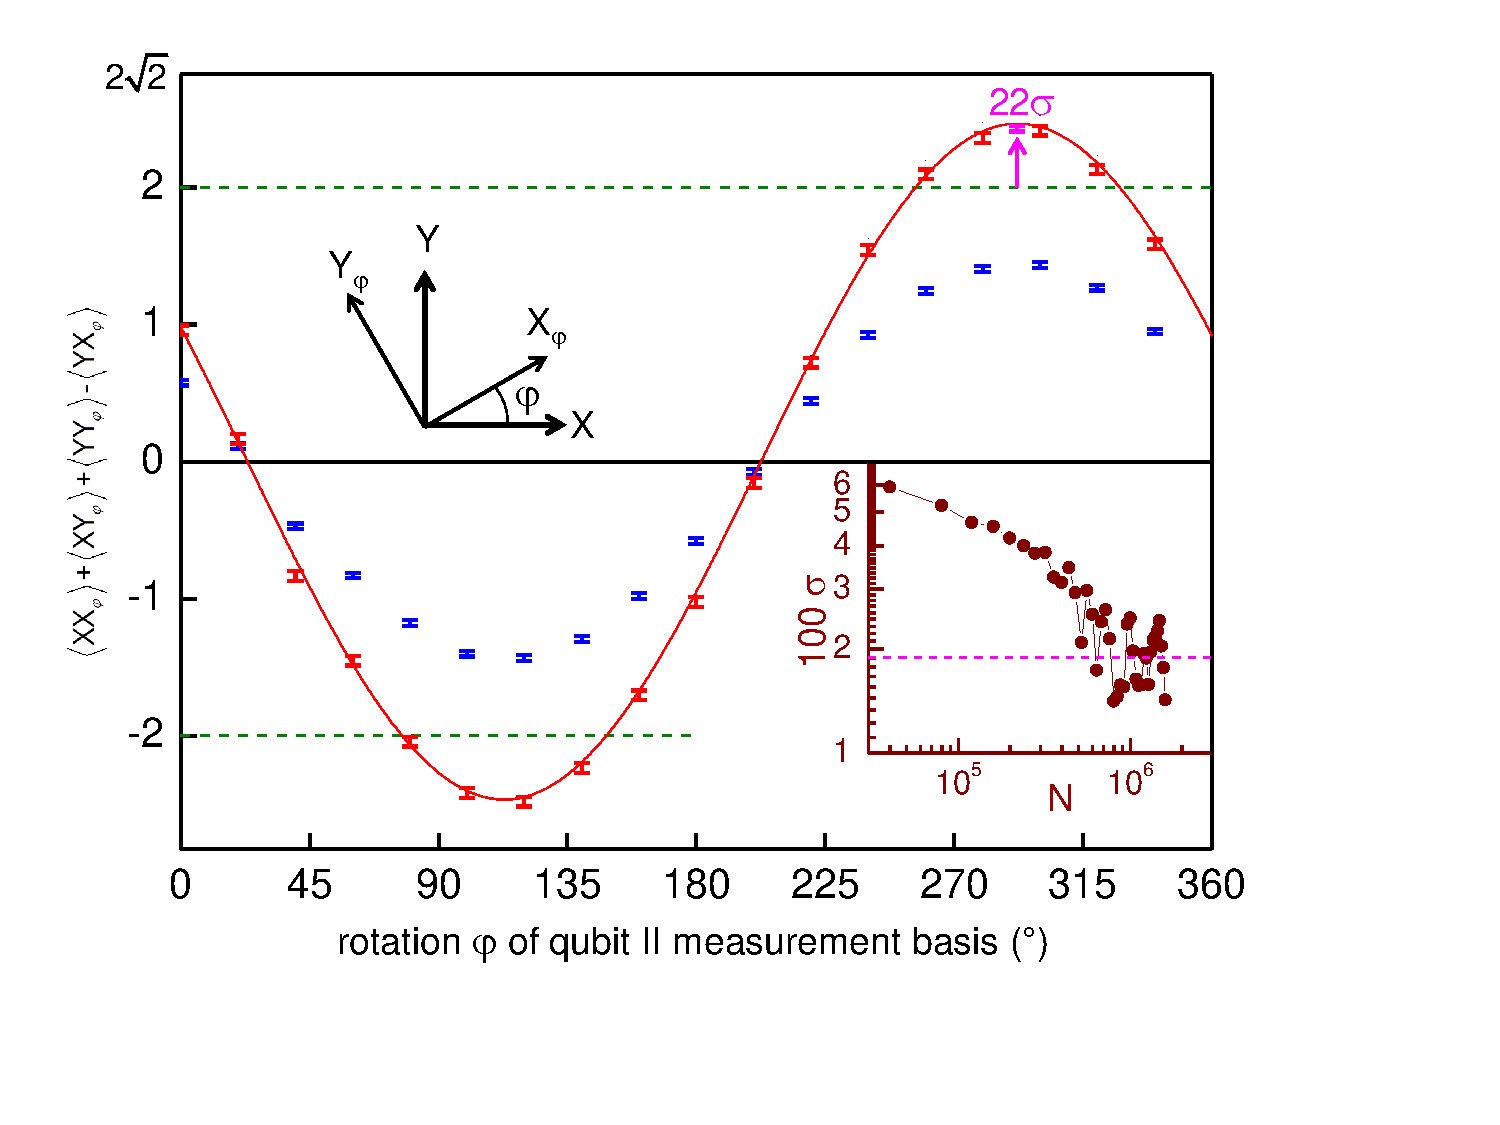
\includegraphics[width=0.8\textwidth]{./material/papers/iswap/figures/chsh}
	\caption[]{Value of the $\bracket{\mathrm{CHSH}}$ operator measured for an ensemble of identically prepared Bell states $1/\sqrt{2}(\ket{01}+e^{-i\varphi}\ket{10})$, plotted as a function of the rotation $\phi$ of the measurement basis. Blue markers correspond to raw measurement data, red markers to data corrected for readout errors. The solid line represents the best fit to the theory. The inset shows the standard deviation $\sigma$ of the maximum value of the $\bracket{\mathrm{CHSH}}$ operator as a function of the sample size. For large samples, $\sigma$ is limited by experimental drift of the measurement basis.}
	\label{fig:chsh}
\end{figure}

\subsubsection{Errors} 

Besides obvious readout errors, the main source of errors in our experiment is drift of the measurement equipment. Most importantly, the phase of the arbitrary waveform generator (AWG) can drift in respect to the phases of the microwave sources, thereby changing the effective phase of the measurement basis of the CHSH operator. Fig. \ref{fig:chsh_drift} illustrates the effect of this drift on the phase of the generated Bell state. Shown is the phase of the state $\ket{\phi}$ as given by eq. (\ref{eq:chsh_state}) extracted from a full CHSH data set as shown in fig. \ref{fig:chsh}. When repeating this measurement over a long time period, oscillations of the phase $\varphi$ with an amplitude of $\approx 40^\circ$ can be observed. This amplitude can be explained by a time shift of the AWG waveform driving the microwave sources of the order of $200\;\mathrm{ps}$, which has indeed been observed experimentally.

\begin{SCfigure}[1.0][hb!]
	\centering
	\includegraphics[width=9cm]{"./data/ct5/2011_03_17 - chsh/chsh_drift"}
	\caption[]{Phase $\varphi$ of an experimentally generated Bell state as a function of time. The phase exhibits oscillatory drift of the order of $\approx 40^\circ$ being caused by a time offset drift of the AWG.}
	\label{fig:chsh_drift}
\end{SCfigure}


\subsection{Measuring the Evolution of an Entangled Qubit States}

\begin{figure}[ht!]
   \centering
	 \includegraphics[width=1.\textwidth]{"./data/ct5/film of swap/pauli_set_vs_time_with_simulation"}
	 \caption[test]{Measured Pauli operators $\sigma_i \otimes \sigma_j$ with $i,j \in \{X,Y,Z,I\}$ as a function of the interaction time. Shown are the 6 single-qubit operators as well as the 9 two-qubit correlation operators. The dashed line represents a master-equation simulation of the experiment.}
	 \label{fig:swap_pauli_set_vs_time_with_simulation}
\end{figure}

Using quantum state tomography, we can repeat the swapping experiment described in section \ref{section:creation_of_entanglement} and reconstruct the full experimental density matrix of our system at many different times during the swap sequence. Like this we can follow the evolution of the quantum state during the course of the swap. Fig. \ref{fig:swap_pauli_set_vs_time_with_simulation} shows the result of such an experiment. We plot the measured values of all Pauli operators as a function of the swapping time between the qubits. The red and green curves correspond to the single-qubit Pauli operators $\sigma^I_{X,Y,Z}\otimes \mathrm{I}$ and $\mathrm{I}\otimes \sigma^{II}_{X,Y,Z}$, the blue curves to the two-qubit Pauli operators $\sigma_{X,Y,Z}^I\otimes \sigma_{X,Y,Z}^{II}$. The dashed line corresponds to a master equation simulation of the swapping experiment, where the qubit coupling, relaxation and dephasing parameters are chosen in accordance with experimental values. As can be seen, the simulation agrees well with the experimental data. Deviation between data and simulation can be seen in the $\sigma_{X,Y}^I\otimes \sigma_{X,Y}^{II}$ operators and is caused by an additional phase acquired by the qubits during the swap. This phase appears due to the fact that we have to shift the frequency of the qubits to bring them in resonance, hence we acquire a dynamical phase in the frame rotating at the uncoupled qubit frequencies. In addition, experimental drift of our measurement equipment may induce an additional phase factor during the measurement, which takes several hours to complete.

\smallskip

From the measured Pauli set, we can reconstruct the density matrix of the two-qubit system at any point during the swap. This density matrices are (will be soon :) shown in the margins of this thesis book. When following the evolution of the quantum state as a function of time (by flipping the pages of the book) it can be seen that the coherence between the two qubits decreases steadily during the swapping sequence, due to relaxation and dephasing.

\section{Realizing a Two-Qubit Gate}

We have demonstrated that it is possible to create highly entangled qubit states with our processor by preparing Bell states, performing quantum state tomography and violating the Bell inequality. However, to realize a universal two-qubit quantum processor, it is necessary to implement a so-called {\it universal two-qubit gate} on our processor. In the following sections we discuss how we can realize and characterize such a gate.

\subsection{Principle}

By definition, a universal two-qubit gate together with a set of universal one-qubit gates, allows us to create any possible two-qubit quantum state \citep{barenco_elementary_1995}. In principle, there are (infinitely) many choices for possible universal two-qubit gates. In this work, we are interested mainly in the so-called $\sqrt{i\mathrm{SWAP}}$ gate, which has the representation
%
\begin{equation}
U(t)=\left(\begin{array}{cccc}
1 & 0 & 0 & 0\\
0 & 1/\sqrt{2} & i/\sqrt{2} & 0\\
0 & i/\sqrt{2} & 1/\sqrt{2} & 0\\
0 & 0 & 0 & 1\end{array}\right)_{\left\{ \left|00\right\rangle ,\left|01\right\rangle ,\left|10\right\rangle ,\left|11\right\rangle \right\} } \label{eq:sqrt_iswap_gate_main}
\end{equation}
%
We can implement this gate naturally using the swapping interaction as given by eq. (\ref{eq:swap_evolution_operator_main}) when letting the qubits evolve in resonance for a time $t_{\sqrt{i\mathrm{SWAP}}}=1/8g$, which, for our experimental value of $2g = 8.3\;\mathrm{MHz}$ corresponds to $t_{\sqrt{i\mathrm{SWAP}}}=30\;\mathrm{ns}$. 

\subsection{Experimental Implementation}

Figure \ref{fig:iswap_pulse_sequence} shows the pulse sequence that we use to realize the $\sqrt{i\mathrm{SWAP}}$ gate with our processor for an exemplary input state. In the case shown, we excite the first qubit to the state $\ket{1}$, creating an input state $\ket{10}$. We then tune in resonance the two qubits for a time $t_{\sqrt{i\mathrm{SWAP}}}$. After tuning the qubits out of resonance again, we apply two single-qubit $Z$-gates to compensate the dynamical phases acquired during the swap. Then, we optionally apply single-qubit tomography gates and finally read out the qubit state at the optimal readout working point. Using this technique we can reconstruct the density matrix of the quantum state after applying the two-qubit gate to it. Similarily, we can perform quantum state tomography on the input state to obtain its density matrix. Reconstructing the input and output density matrices for a range of different input state will then allow us to fully characterize the gate operation, as will be discussed in the next section.

\begin{figure}[ht!]
	\centering
		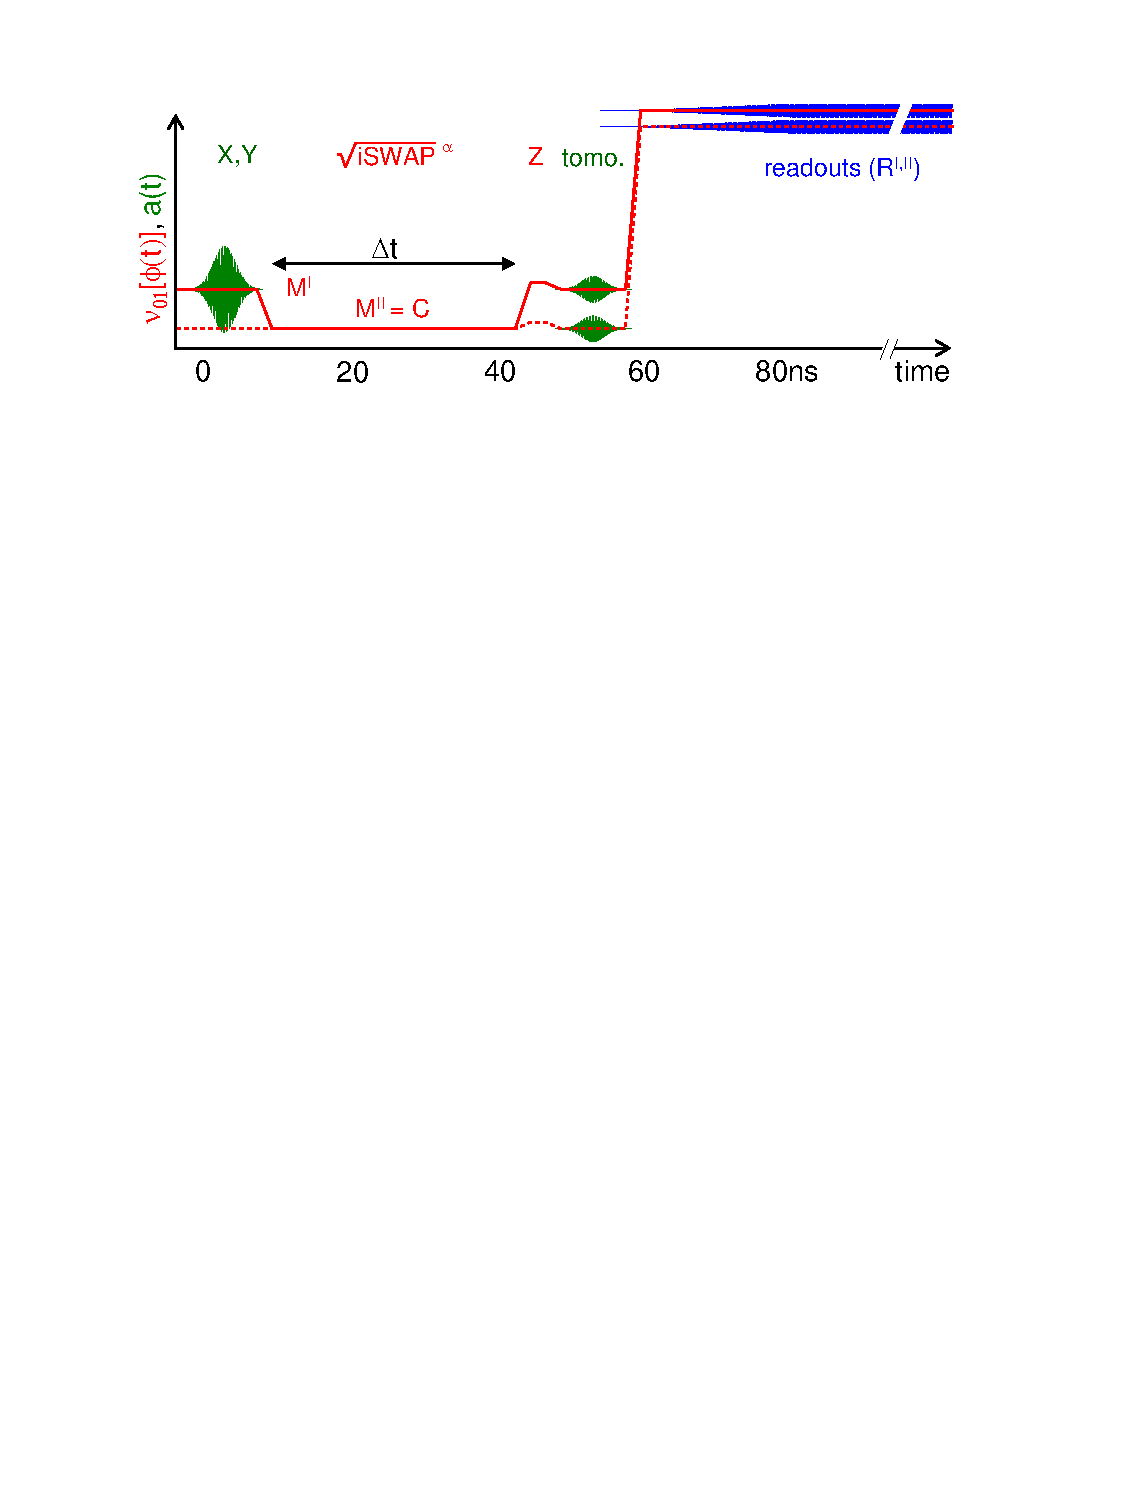
\includegraphics[width=0.8\textwidth]{./material/papers/iswap/figures/iswap_gate_pulse_sequence}
	\caption{Experimental pulse sequence used for implementing the two-qubit $\sqrt{i\mathrm{SWAP}}$ gate. The sequence shown for an exemplary input state $\ket{10}$ consists in exciting the first qubit to the state $\ket{1}$, bringing the qubits in resonance for a time $t=1/8g$, separating them and compensating the acquired dynamical phases by using two single-qubit $Z$-pulses. Finally, optional tomographic pulses are applied before reading out the qubit state at the optimal readout frequencies of the qubits.}
	\label{fig:iswap_pulse_sequence}
\end{figure}


\subsection{Quantum Process Tomography of the Gate}

To characterize the fidelity of our quantum gate, we perform so-called {\it quantum process tomography} \citep{poyatos_complete_1997}. This procedure allows us to fully characterize a quantum process in an open quantum system. The approach that we use in this work is called {\it standard quantum process tomography} (SQPT), however, there exist other common methods such as ancilla-assisted quantum process tomography \citep{dur_nonlocal_2001,dariano_quantum_2001,altepeter_ancilla-assisted_2003}, that we will not discuss since they are not relevant to this work.

\smallskip

In the following section, we will introduce the concept of a quantum process, explain possible parametrizations of such a process and discuss the experimental implementation of standard quantum process tomography on our two-qubit processor.

\subsubsection{Theoretical Description of a Quantum Process}

A quantum process can be described as a function $\mathcal{E} : \rho_\mathcal{H} \to \rho_\mathcal{H}$ that maps a density matrix $\rho$ defined in a Hilbert space $Q_1$ to another density matrix $\mathcal{E}(\rho)$ defined in a target Hilbert space $Q_2$ and that fulfills three axiomatic properties \cite{nielsen_quantum_2000,haroche_exploring_2006}:

\begin{axiom}
$\mathrm{tr}\left[\mathcal{E}(\rho)\right]$ is the probability that the process represented by $\mathcal{E}$ occurs, when $\rho$ is the initial state.
\end{axiom}

\begin{axiom}
$\mathcal{E}$ is a {\it convex-linear map} on the set of density matrices, that is, for probabilities $\left\{p_i\right\}$,

  \begin{equation}
	  \mathcal{E}\left(\sum\limits_i p_i \rho_i\right) = \sum\limits_i p_i \mathcal{E}(\rho_i)
	\end{equation}
\end{axiom}

\begin{axiom}
$\mathcal{E}$ is a {\it completely-positive} map. That is, if $\mathcal{E}$  maps density operators of system $Q_1$ to density operators of system $Q_2$, then $\mathcal{E}(A)$ must be positive for any positive operator $A$. Furthermore, if we introduce an extra system $R$ of arbitrary dimensionality, it must be true that $(\mathcal{I}\otimes \mathcal{E})(A)$ is positive for any positive operator $A$ on the combined system $R\otimes Q_1$, where $\mathcal{I}$ denotes the identity map on system $R$.
\end{axiom}
As shown in \cite{nielsen_quantum_2000}, any quantum process fulfilling these criteria can be written in the form

\begin{equation}
  \mathcal{E}(\rho) = \sum\limits_i E_i \rho E_i^\dagger \label{eq:process_operator_sum_representation}
\end{equation}
for some set of operators $\{ E_i \}$ which map the input Hilbert space to the output Hilbert space, and for which $\sum_i E_i^\dagger E_i \le I$. Here, the operators $E_i$ are called the {\it Kraus operators} of the quantum process. They contain the full information of the quantum process acting on $\rho$.

\smallskip

If we express the operators $E_i$ in a different operator basis $\tilde{E}_j$ such that $E_i = \sum_j a_{ij} \tilde{E}_{j}$ and insert into eq. (\ref{eq:process_operator_sum_representation}), we obtain

\begin{eqnarray}
 \mathcal{E}(\rho) & = & \sum\limits_i \sum\limits_j a_{ij} \tilde{E}_j \;\rho\; \sum\limits_k a_{ik}^* \tilde{E}_k^\dagger \\
& = & \sum\limits_{j,k}\tilde{E}_j \; \rho \; \tilde{E}_k^\dagger \sum\limits_i a_{ij} a_{ik}^* \\
& = & \sum\limits_{j,k}\tilde{E}_j \; \rho \; \tilde{E}_k^\dagger \; \chi_{jk} \label{eq:process_chi_representation}
\end{eqnarray}
where we defined $\chi_{jk} = \sum\limits_i a_{ij} a_{ik}^*$. This is the so-called $\chi$-matrix representation of the quantum process. Here, all the information on the process is contained in the matrix $\chi$, which controls the action of the now process-independent operators $\tilde{E}_i$ on the initial density matrix $\rho$.

\subsubsection{Implementation}

As said before, the goal of QPT is to obtain the coefficients of the $\chi$-matrix -- or any other complete parametrization of the process -- from a set of experimentally measured density matrices $\{\rho_i\}$ and $\{\mathcal{E}(\rho_i)\}$. Standard process tomography \citep{nielsen_quantum_2000,poyatos_complete_1997} can be implemented for our two-qubit gate by using the following procedure:

\begin{enumerate}
\item Choose a set of operators $E_i$ that forms a full basis of $\mathcal{M}: Q_1 \to Q_2$. For n-qubit process tomography we usually choose $E_{i_1,i_2 \hdots i_n} = \sigma_{i_1}\otimes \sigma_{i_2}\hdots\otimes\sigma_{i_n}$, where $\sigma_i$ are the single-qubit Pauli operators and $i\in\{I,X,Y,Z\}$. For a Hilbert space of dimension $n$, this yields $4^n-1$ operators (excluding the trivial operator $I^{\otimes n}$).
\item Choose $4^n$ pure quantum states $\ket{\phi_i}$ such that the basis $\{\ket{\phi_1}\bra{\phi_1},\hdots,\ket{\phi_{4^n}}\bra{\phi_{4^n}}\}$ spans the whole space of input density matrices $\rho$. Usually, for a n-qubit system we choose $\phi = \{\ket{0},\ket{1},(\ket{0}+\ket{1})/\sqrt{2},(\ket{0}+i\ket{1})/\sqrt{2}\}^{\otimes n}$, where $^{\otimes n}$ denotes the n-dimensional Kronecker product of all possible permutations.
\item For each of the $\ket{\phi_i}$, determine $\mathcal{E}(\ket{\phi_i}\bra{\phi_i})$ by quantum state tomography. Usually we also determine $\ket{\phi_i}\bra{\phi_i}$ experimentally since the preparation of this state already entails small preparation errors that should be taken into account when performing quantum process tomography. 
\end{enumerate}

After having obtained the $\rho_i$ and $\mathcal{E}(\rho_i)$ one obtains the $\chi$-matrix by writing $\mathcal{E}(\rho_i) = \sum_j \lambda_{ij} \tilde{\rho}_j$, with some arbitrary basis $\tilde{\rho}_j$ and
letting $\tilde{E}_m \tilde{\rho}_j \tilde{E}_n^\dagger = \sum_k \beta_{jk}^{mn}\tilde{\rho}_k$. We can then insert into eq. (\ref{eq:process_chi_representation}) and obtain
\begin{eqnarray}
\sum\limits_k \lambda_{ik} \tilde{\rho}_k & = & \sum\limits_{m,n} \chi_{mn} \sum\limits_k \beta_{ik}^{mn} \tilde{\rho}_k  
\end{eqnarray}
This directly yields $\lambda_{ik} = \sum_{m,n}\beta_{ik}^{mn}\; \chi_{mn}$, which, by linear inversion,  gives $\chi$. Hence, we can fully characterize a quantum process acting on an $n$-dimensional Hilbert space by measuring $2\cdot 4^n$ experimental density matrices (or $4^n$ when assuming that no errors occur during the preparation of the input states, which thereby are known).

\smallskip

Similar to quantum state tomography, experimental errors occurring during quantum process tomography can produce a set of process parameters $\chi$ that are {\it non-physical} in the sense that the resulting quantum process does not obey the three axioms stated above. We can resolve this problem by rendering the obtained $\chi$ matrix physical by a standard mathematical procedure. When doing this, we usually choose the  physical $\chi_{ph}$ matrix that has the smallest distance $d=\|\chi-\chi_{ph}\|$.

\subsubsection{From the $\chi$ matrix to the Kraus representation}

To go back from the $\chi$-matrix representation of the quantum process to the Kraus form we write each process-independent operator $\tilde{E}_i$ as a sum of all the Kraus operators $E_l$, such that
%
\begin{equation}
	\tilde{E}_i = \sum\limits_l a_{il}\; E_l
\end{equation}
%
Inserting this into eq. (\ref{eq:process_chi_representation}) we obtain
%
\begin{eqnarray}
\begin{mathcal}E\end{mathcal}(\rho) & = & \sum\limits_{j,k}\chi_{jk}\sum\limits_{l,m} a_{jl}a_{km}^* E_l \rho E_m^\dagger   \label{eq:process_chi_transformed} \\
& = & \sum\limits_i E_i \rho E^\dagger_i
\end{eqnarray}
%
We find hence that $\sum\limits_{j,k} \chi_{jk}a_{jl}a_{km}^* = \delta_l^m$, or, written in matrix form $A\chi A^\dagger = \mathrm{I}$. This identity is true for $A$ being the matrix of eigenvectors of $\chi$, multiplied by the square root of the corresponding matrix of eigenvalues. It is thus easy to obtain the Kraus representation of the quantum process by diagonalizing the Hermitian matrix $\chi$.

\smallskip

The Kraus operator form of the quantum process is useful since it allows us to easily visualize the different operators acting on the density matrix $\rho$. By ordering the Kraus operators in function of their associated eigenvalues we can easily visualize the different unitary and non-unitary processes acting together on the density matrix $\rho$.

\subsubsection{Experimental Results: Input/Output Matrices And $\chi$-Matrix}

\begin{figure}[p]
	\centering
		\includegraphics[width=1.0\textwidth]{"./data/ct5/2011_04_21 - grover and tomo/good_data/process -matrices 1"}
	\caption{The experimental input-output density matrices of the quantum process tomography of the $\sqrt{i\mathrm{SWAP}}$ gate. Shown are the measured density matrices of 16 different input states and the corresponding output matrices with their state fidelities. The ideal matrices are overlaid in black. (part I/II)}
	\label{fig:process_matrices_1}
\end{figure}

\begin{figure}[p]
	\centering
		\includegraphics[width=1\textwidth]{"./data/ct5/2011_04_21 - grover and tomo/good_data/process -matrices 2"}
	\caption{The experimental input-output density matrices of the quantum process tomography of the $\sqrt{i\mathrm{SWAP}}$ gate. Shown are the measured density matrices of 16 different input states and the corresponding output matrices with their state fidelities. The ideal matrices are overlaid in black. (part II/II)}
	\label{fig:process_matrices_1}
\end{figure}

We perform standard process tomography of our two-qubit gate by following the procedure outlined in the last sections. Figs. \ref{fig:process_matrices_1} and \ref{fig:process_matrices_1} summarize the experimentally determined input-output density matrices, measured for our two-qubit $\sqrt{i\mathrm{SWAP}}$ quantum gate. We show pairs of corresponding input and output states together, containing both the reconstructed experimental density matrices as well as the ideal density matrices. The ideal input states are annotated below the corresponding density matrices. Above each matrix we show the trace fidelity between it and the ideal quantum state. A total of 16 input/output pairs has been measured, corresponding to a complete set of states necessary to fully characterize the quantum process of our gate operation.

\smallskip

\begin{figure}[ht!]
	\centering
		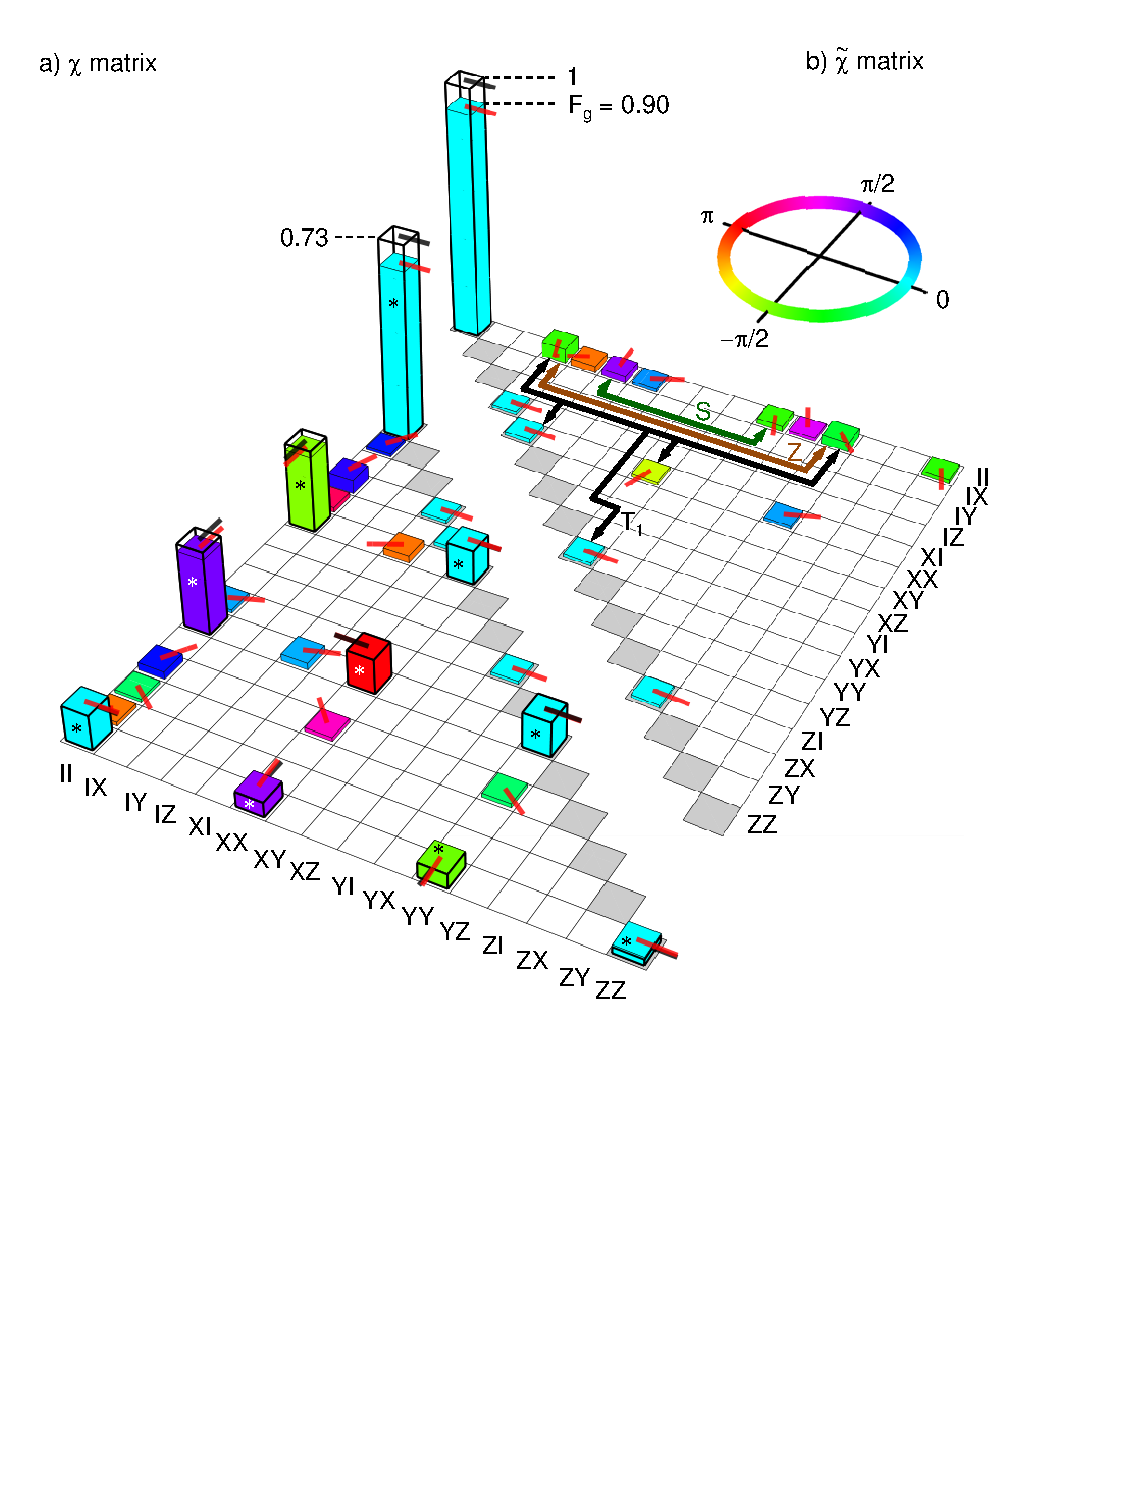
\includegraphics[width=1.\textwidth]{./material/papers/iswap/figures/chi_matrix_and_error_process}
	\caption{The reconstructed $\chi$ matrix of our implementation of the $\sqrt{i\mathrm{SWAP}}$ quantum gate. a) shows the lower half of the Hermitian matrix is shown. b) shows the product $\tilde{\chi}=\chi\cdot\chi_{id}^{-1}$ of the measured $\chi$ matrix and the ideal process matrix $\chi_{id}$. The colored arrows connecting different elements of $\tilde{\chi}$ indicate unitary and non-unitary error processes to which the corresponding matrix elements can be associated.}
	\label{fig:chi_matrix_and_errors}
\end{figure}

From these input/output matrices, we can easily calculate the $\chi$ matrix of the quantum process by the method described above. The resulting matrix is shown in fig. \ref{fig:chi_matrix_and_errors}. There, we show the experimentally obtained $\chi$ matrix of our $\sqrt{i\mathrm{SWAP}}$ gate as well as the error process defined as $\tilde{\chi} = \chi\cdot\chi_{id}$, where $\chi_{id}$ corresponds to the ideal gate process. $\chi_{id}$ is as well shown as black outlines overlaid to the measured $\chi$ matrix. The arrows connecting different parts of the $\tilde{\chi}$ matrix group several unitary and non-unitary error processes that can be attributed to the individual elements.

\subsection{Gate Fidelity}

After having obtained the experimental $\chi$ matrix, it is trivial to calculate the process fidelity, which is defined as $F=\mathrm{Tr}\{\chi_{id}\cdot\chi\}$, where $\chi_{id}$ corresponds to the ideal quantum process. For our experimental process matrix, it is given as $F=0.9$. The fidelity can be roughly compared to the output state fidelity averaged over the whole set of possible input density matrices.

\subsection{Gate Error Analysis}

We treat two classes of errors in our analysis: Unitary and non-unitary gate errors as well as tomography errors. The former are associated to errors in the quantum process itself, whereas the latter are caused by unitary and non-unitary errors during quantum state tomography.

\smallskip

\subsubsection{Tomographic Errors} \label{section:tomographic_errors}

Tomographic errors are removed from the process map of our $\sqrt{iSWAP}$
gate using the following method: The measured Pauli sets corresponding
to the sixteen input states are first fitted by a model including
errors both in the preparation of the state (index $prep$) and in
the tomographic pulses (index $tomo$). The errors included are angular
errors $\varepsilon_{\mathrm{I,II}}^{\mathrm{prep}}$ on the nominal
$\pi$ rotations around $X_{\mathrm{I,II}}$, $\eta_{\mathrm{I,II}}^{\mathrm{prep,tomo}}$and
$\delta_{\mathrm{I,II}}^{\mathrm{prep,tomo}}$ on the nominal $\pi/2$
rotations around $X_{\mathrm{I,II}}$ and $Y_{\mathrm{I,II}}$, a
possible departure $\xi_{\mathrm{I,II}}$ from orthogonality of $\left(\overrightarrow{X_{\mathrm{I}}},\overrightarrow{Y_{\mathrm{I}}}\right)$
and $\left(\overrightarrow{X_{\mathrm{II}}},\overrightarrow{Y_{\mathrm{II}}}\right)$,
and a possible rotation $\mu_{\mathrm{I,II}}$ of the tomographic
$XY$ frame with respect to the preparation one. The rotation operators
used for preparing the states and doing their tomography are thus
given by

\[
\begin{array}{c}
X_{\mathrm{I,II}}^{\mathrm{prep}}(\pi)=e^{-\mathrm{i}\left(\pi+\varepsilon_{\mathrm{I,II}}^{\mathrm{prep}}\right)\sigma_{\mathrm{x}}^{\mathrm{I,II}}/2},\\
X_{\mathrm{I,II}}^{\mathrm{prep}}(-\pi/2)=e^{+\mathrm{i}\left(\pi/2+\eta_{\mathrm{I,II}}^{\mathrm{prep}}\right)\sigma_{\mathrm{x}}^{\mathrm{I,II}}/2},\\
Y_{\mathrm{I,II}}^{\mathrm{prep}}(\pi/2)=e^{-\mathrm{i}\left(\pi/2+\delta_{\mathrm{I,II}}^{\mathrm{prep}}\right)\left[\mathrm{cos}\left(\xi_{\mathrm{I,II}}\right)\sigma_{\mathrm{y}}^{\mathrm{I,II}}\mathrm{-sin}\left(\xi_{\mathrm{I,II}}\right)\sigma_{\mathrm{x}}^{\mathrm{I,II}}\right]/2},\\
X_{\mathrm{I,II}}^{\mathrm{tomo}}(\pi/2)=e^{-\mathrm{i}\left(\pi/2+\eta_{\mathrm{I,II}}^{\mathrm{tomo}}\right)\left[\mathrm{\mathrm{sin}\left(\mu_{I,II}\right)\sigma_{x}^{I,II}+cos}\left(\mu_{\mathrm{I,II}}\right)\sigma_{\mathrm{y}}^{\mathrm{I,II}}\right]/2},\\
Y_{\mathrm{I,II}}^{\mathrm{tomo}}(-\pi/2)=e^{+\mathrm{i}\left(\pi/2+\delta_{\mathrm{I,II}}^{\mathrm{tomo}}\right)\left[\mathrm{cos}\left(\mu_{\mathrm{I,II}}+\xi_{\mathrm{I,II}}\right)\sigma_{\mathrm{y}}^{\mathrm{I,II}}\mathrm{-sin}\left(\mu_{\mathrm{I,II}}+\xi_{\mathrm{I,II}}\right)\sigma_{x}^{\mathrm{I,II}}\right]/2}.\end{array}\]
The sixteen input states are then $\{ \rho_{\mathrm{in}}^{\mathrm{e}}=U\left|0\right\rangle \left\langle 0\right|U^{\dagger}\} $
with 
%
\begin{equation}
\{ U\} =\{I_{\mathrm{I}}, X_{\mathrm{I}}^{\mathrm{prep}}(\pi), Y_{\mathrm{I}}^{\mathrm{prep}}(\pi/2),X_{\mathrm{I}}^{\mathrm{prep}}(-\pi/2)\}\otimes\{I_{\mathrm{II}},X_{\mathrm{II}}^{\mathrm{prep}}(\pi),Y_{\mathrm{II}}^{\mathrm{prep}}(\pi/2),X_{\mathrm{II}}^{\mathrm{prep}}(-\pi/2)\},
\end{equation}
%
and each input state yields a Pauli set $\left\{ \left\langle P_{\mathrm{k}}^{\mathrm{e}}\right\rangle =Tr\left(\rho_{\mathrm{in}}^{\mathrm{e}}P_{\mathrm{k}}^{\mathrm{e}}\right)\right\} $
with $\left\{ P_{\mathrm{k}}^{\mathrm{e}}\right\} =\{I_{\mathrm{I}},X_{\mathrm{I}}^{\mathrm{e}},Y_{\mathrm{I}}^{\mathrm{e}},Z_{\mathrm{I}}\}\otimes\{I_{\mathrm{II}},X_{\mathrm{II}}^{\mathrm{e}},Y_{\mathrm{II}}^{\mathrm{e}},Z_{\mathrm{II}}\}$,
$X^{\mathrm{e}}=Y^{\mathrm{tomo}}(-\pi/2)^{\dagger}\sigma_{z}Y^{\mathrm{tomo}}(-\pi/2)$,
and $Y^{\mathrm{e}}=X^{\mathrm{tomo}}(\pi/2)^{\dagger}\sigma_{\mathrm{z}}X^{\mathrm{tomo}}(\pi/2)$.
The best fit to the modeled $\left\{ \left\langle P_{k}^{e}\right\rangle \right\} $
set to the measured input Pauli sets yields $\varepsilon_{\mathrm{I}}^{\mathrm{prep}}=-1\text{\textdegree}$,
$\varepsilon_{\mathrm{II}}^{\mathrm{prep}}=-3\text{\textdegree}$,
$\eta_{\mathrm{I}}^{\mathrm{prep}}=3\text{\textdegree}$, $\mathrm{\eta}_{\mathrm{II}}^{\mathrm{prep}}=4\text{\textdegree}$,
$\delta_{\mathrm{I}}^{\mathrm{prep}}=-6\text{\textdegree}$, $\delta_{\mathrm{II}}^{\mathrm{prep}}=-3\text{\textdegree}$,
$\eta_{\mathrm{I}}^{\mathrm{tomo}}=-6\text{\textdegree}$, $\eta_{\mathrm{II}}^{\mathrm{tomo}}=-4\text{\textdegree}$,
$\lambda_{\mathrm{I}}^{t\mathrm{omo}}=12\text{\textdegree}$, $\lambda_{\mathrm{II}}^{\mathrm{tomo}}=5\text{\textdegree}$,
$\xi_{\mathrm{I}}=1\text{\textdegree}$, $\xi_{\mathrm{II}}=-2\text{\textdegree}$,
and $\mu_{\mathrm{I}}=\mu_{\mathrm{II}}=-11\text{\textdegree}$.

Knowing the tomographic errors and thus $\left\{ \left\langle P_{\mathrm{k}}^{\mathrm{e}}\right\rangle \right\} $,
we then invert the linear relation $\left\{ \left\langle P_{\mathrm{k}}^{\mathrm{e}}\right\rangle =Tr\left(\rho P_{\mathrm{k}}^{\mathrm{e}}\right)\right\} $
to find the $16\times16$ matrix $B$ that links the vector $\overrightarrow{\left\langle P_{\mathrm{k}}^{\mathrm{e}}\right\rangle }$
to the columnized density matrix $\overrightarrow{\rho}$, i.e. $\overrightarrow{\rho}=B.\overrightarrow{\left\langle P_{\mathrm{k}}^{\mathrm{e}}\right\rangle }$.
The matrix $B$ is finally applied to the measured sixteen input and
sixteen output Pauli sets to find the sixteen $(\rho_{\mathrm{in},},\rho_{\mathrm{out}})_{\mathrm{k}}$
couples to be used for calculating the gate map.

\subsubsection{Unitary and Non-Unitary Gate Errors}

After having eliminated the tomography errors, only gate errors remain. These can be unitary or non-unitary errors occuring during the quantum process. We characterize both of these errors by fitting the experimental $\chi$ matrix to a master equation model of the quantum process which includes unitary (a frequency offset when performing the swapping interaction and phase errors in the compensating $Z$ pulses applied after the swap) and non-unitary (qubit relaxation and dephasing during the whole process). Typically, the relaxation and dephasing rates employed in the simulation are chosen in accordance with experimentally measured $T_1$ and $T_2$ times (taking into account possible renormalizations of these coefficients). On the other side, the unitary error parameters are used as fitting parameters to maximize the fidelity between the experimentally measured process matrix $\chi$ and the simulated one $\chi_{sim}$. Using this technique, we can calculate an error budget of the quantum process that quantifies the contributions of individual error sources. For our process, we find a total gate error of $10 \%$, where we can attribute $8\%$ of the errors to relaxation and decoherence during the process and $2\%$ to unitary gate errors. In principle, after having characterized the unitary gate errors occurring during the process we could, in theory, compensate them in our experiment. However, due to fast drift of the qubit parameters during the experiment we usually do not perform this kind of optimal qubit control to our gate. Under certain circumstances, the effect of non-unitary errors can also be compensated or alleviated by adding or modifying the unitary gate sequence during the quantum process (see e.g. \citep{lange_universal_2010}). However, this procedure is in general not applicable to arbitrary quantum processes and is not applicable to this work.
